\section{Algorithms Applicable to Graphs}
\label{sec:algorithms}

Algorithms for analyzing pathways and networks have been placed  into three main categories by~\cite{Khatri2012}: \ac{ORA}, \ac{FCS}, and \ac{PT}.
\ac{ORA} often focuses on the number of differentially expressed genes present or absent in a gene set compared to chance, while \ac{FCS} is less susceptible to large effects and considers the aggregate of groups of small effects.
\ac{PT} finally considers the biological relations between members of the pathway during analysis.

\subsection{BEL Algorithms}
\label{subsec:bel_algorithms}

Furthermore, Martin \textit{et al.} made the distinction between methods that rely on the assumption that protein activities are correlated with their corresponding mRNAs' expression changes (forward reasoning) versus the effect that upstream controllers of mRNA expression have (backwards reasoning)~\cite{Martin2014}.
These algorithms have been developed for a wide variety of applications, data formats, and graph types.
While many are heterogeneous, below are the most notable algorithms specific to networks from knowledge assemblies encoded in BEL.

\subsubsection{Reverse Causal Reasoning}

Reverse causal reasoning (\ac{RCR}) is an approach to identify the upstream controllers of biological patterns measured in an experiment; often differential gene expression experiments between healthy and diseased patients.
First, large knowledge assemblies are dissected into smaller hypothesis networks with one upstream node with multiple outgoing causal relations to target nodes represented by the experimental data set.
Each hypothesis network is scored by its concordance between the observed up- and down-regulations of targets nodes to the sign of the causal relation and by its richness, or the explanatory power of the hypothesis network~\cite{Catlett2013}.
An example hypothesis network is shown in Figure~\ref{fig:rcr_schematic}.

\begin{figure}
\captionsetup{format=plain}
\makebox[\textwidth]{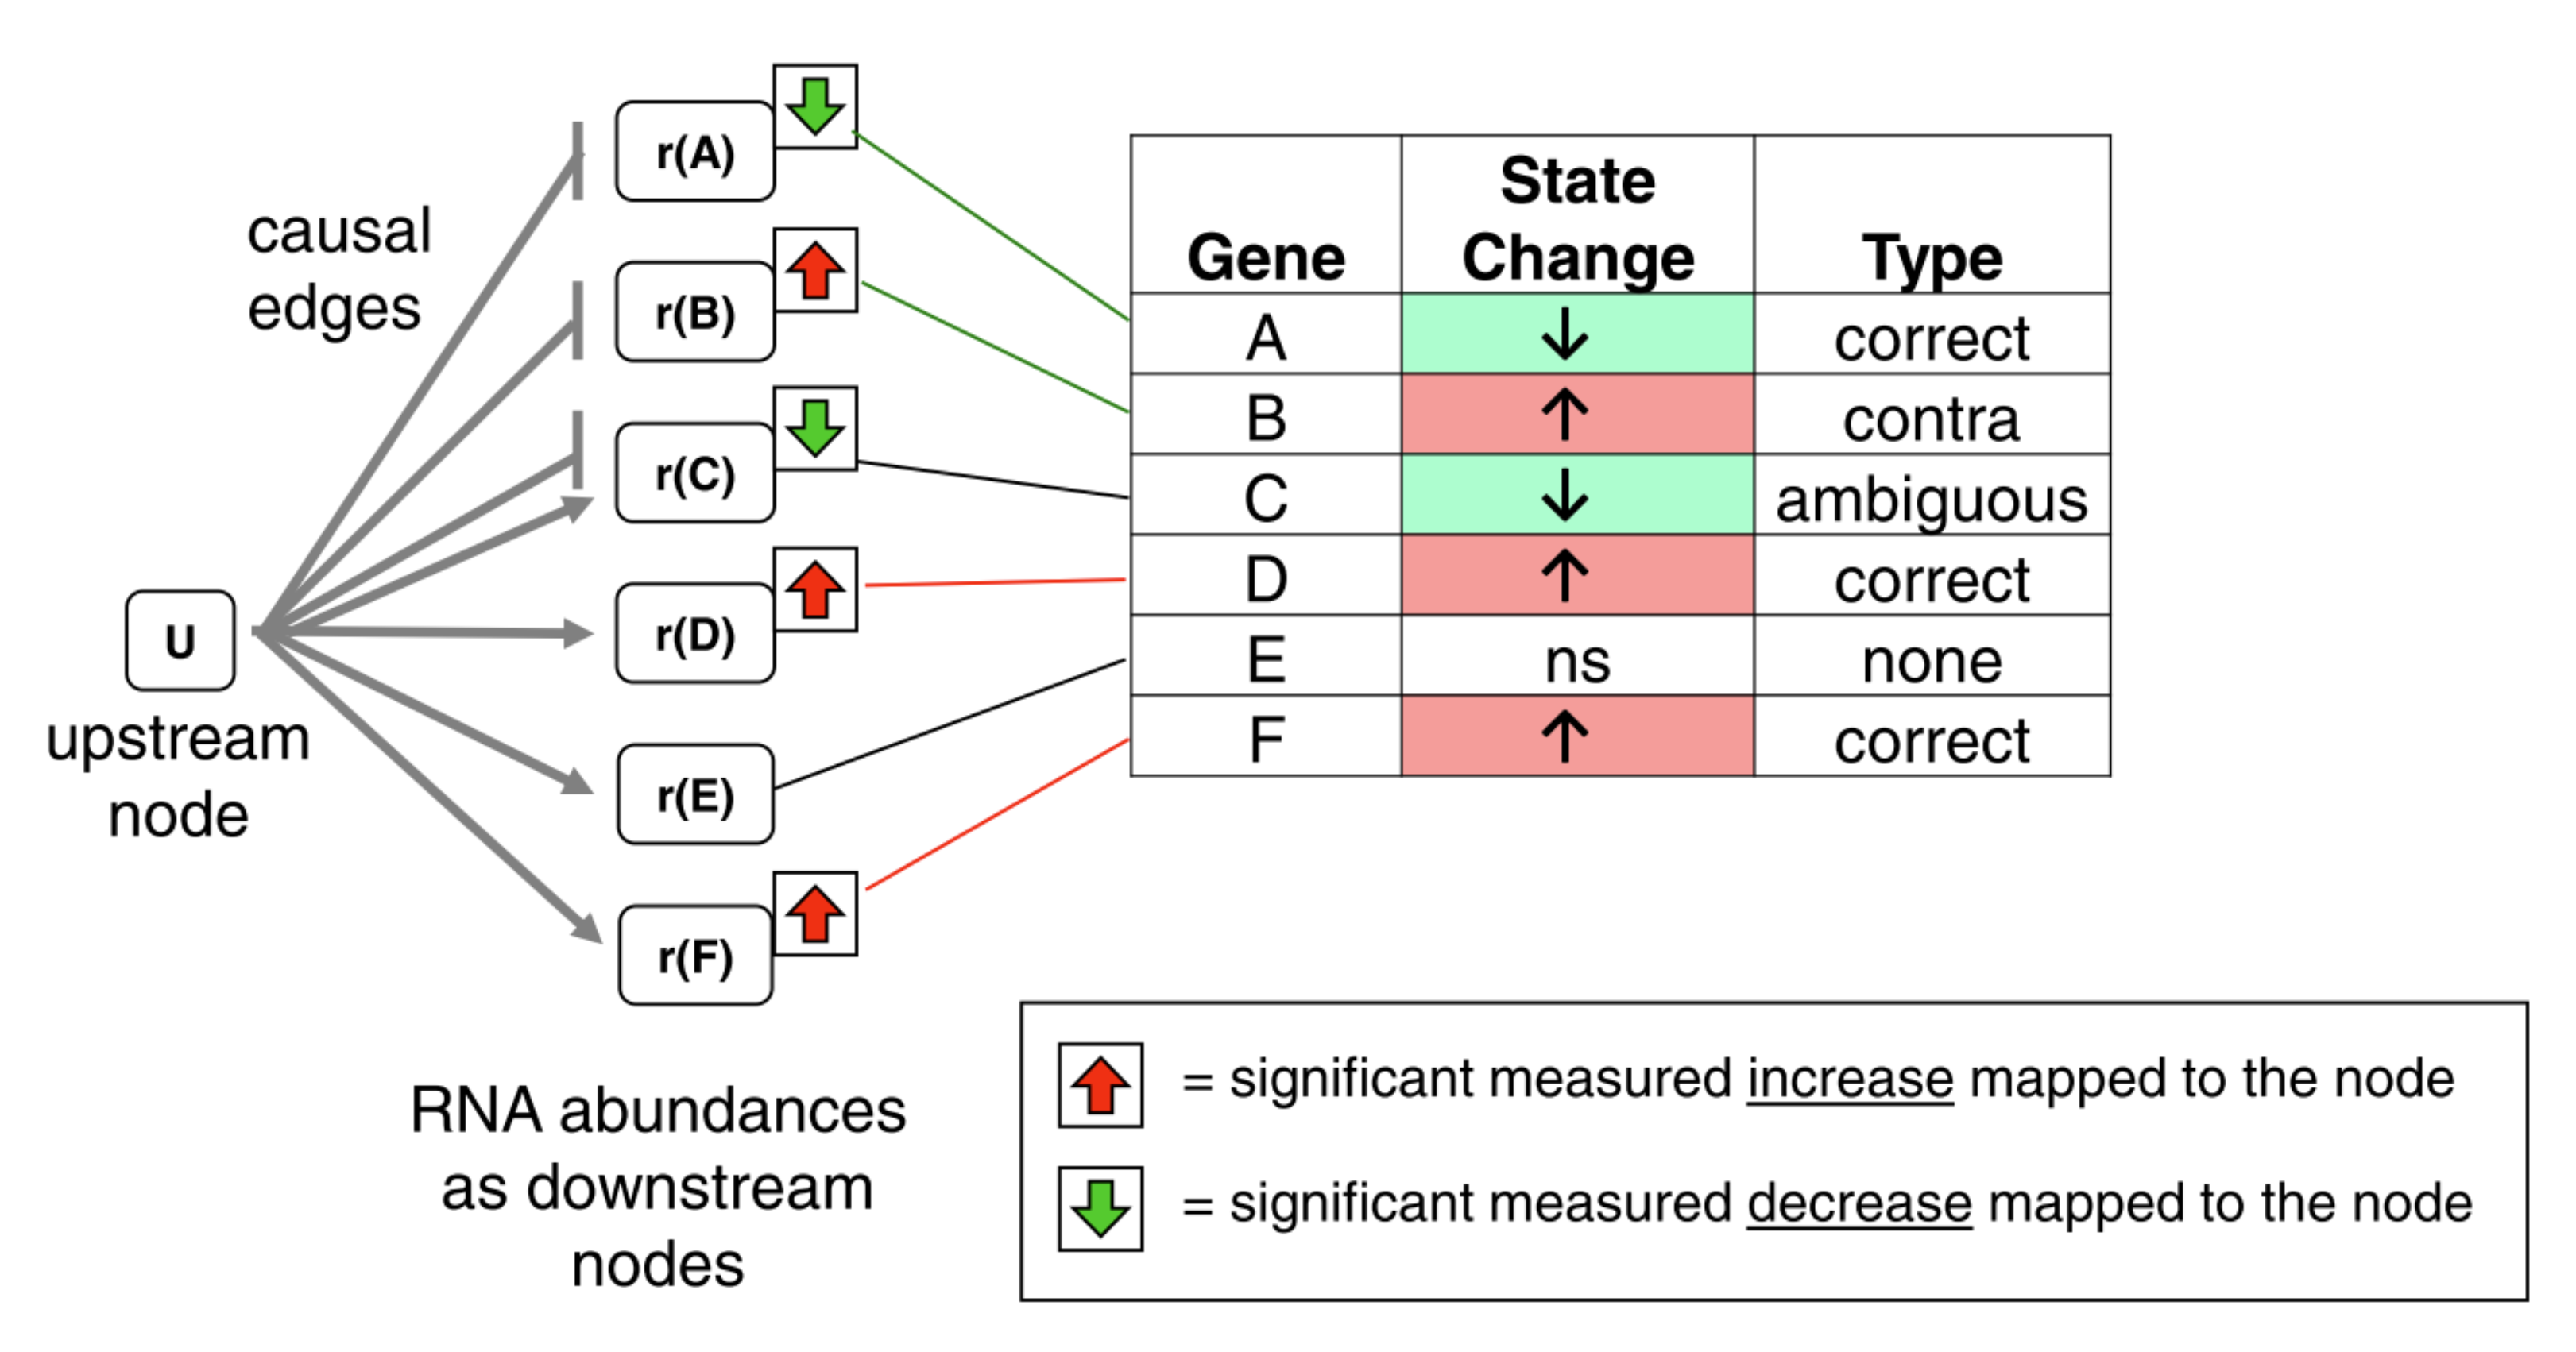
\includegraphics[width=160mm]{figures/rcr_schematic.png}}
\caption[A Schematic Diagram of \ac{RCR}]{An example hypothesis network. Target nodes are counted as correct if they have a decreasing relationship and down-regulation, or an increasing relationship and up-regulation. Target nodes with multiple conflicting relationships are marked as ambiguous. Finally, target nodes are counted as incorrect if they have a mismatch between an increasing relationship and down-regulation, or a decreasing relationship and up-regulation. Adapted from~\cite{Catlett2013}.}
\label{fig:rcr_schematic}
\end{figure}

\subsubsection{Network Perturbation Amplitude}

While \ac{RCR} gives preliminary insights to significant biological controllers, it mostly ignores the topology of signaling, regulatory, and other causal networks that can be represented in knowledge assemblies (Figure~\ref{fig:npa_schematic}).
The \ac{NPA} measures the aggregated effect explained by the controller layer with reference to a given node with respect to their downstream nodes.
Two complementary statistics for the effect of permutations of the upstream layer and downstream layer allow for further insight to the validity of \ac{NPA}s as a hypothesis generation mechanism~\cite{Martin2014}.

\begin{figure}
\captionsetup{format=plain}
\makebox[\textwidth]{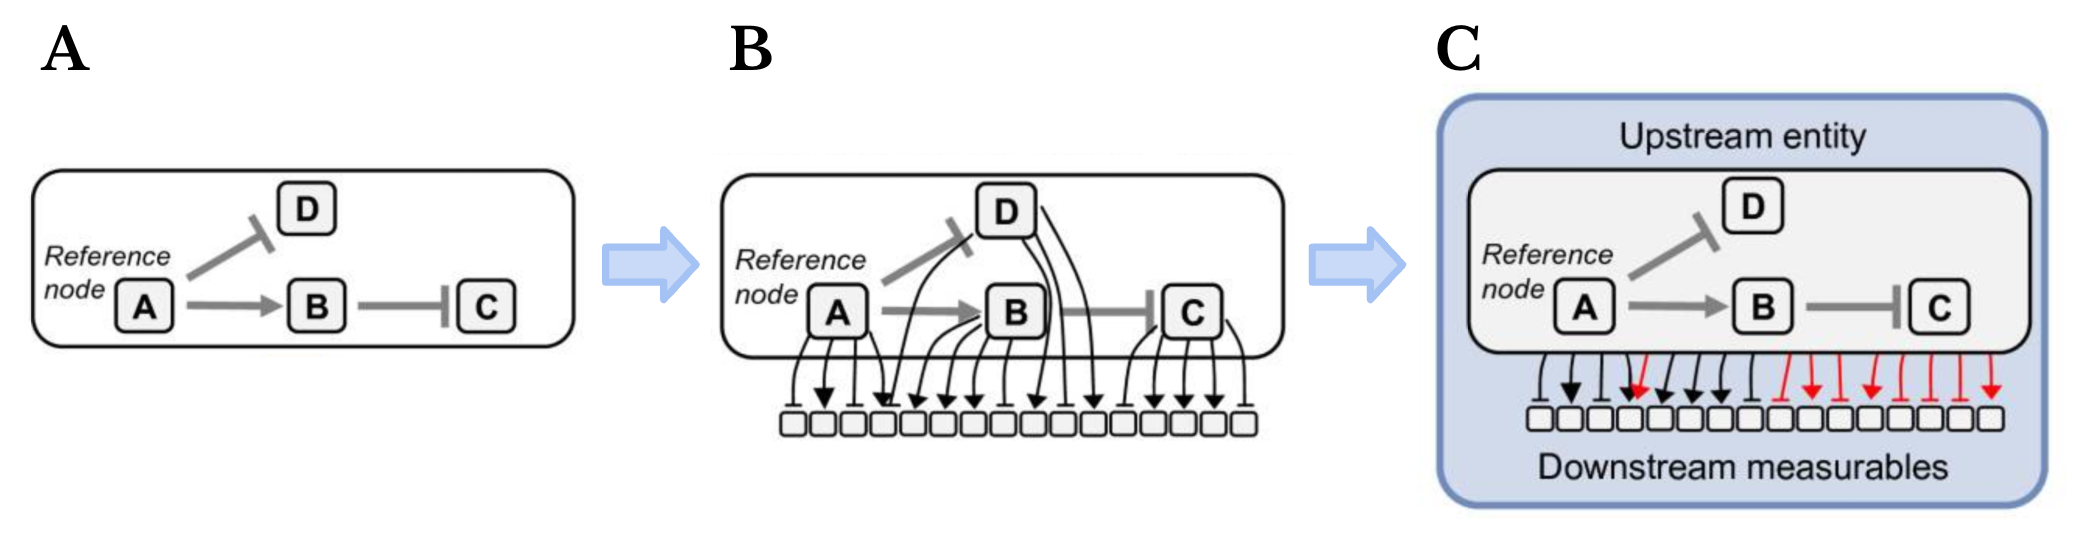
\includegraphics[width=160mm]{figures/npa_schematic.png}}
\caption[Hypothesis Network Generation for \ac{NPA}]{Creation of hypothesis networks that accounts for the topology and interactions of  upstream controller layer with respect to a reference node A), their individual effects on the downstream layer B) and their combine effect C). Adapted from~\cite{Martin2012}.}
\label{fig:npa_schematic}
\end{figure}

\subsubsection{Sampling of Spanning Trees}

While \ac{NPA} enables more informed analyses than \ac{RCR}, its mathematical basis limits the topologies of knowledge networks that can be used to those with causal consistency.
In these networks, all paths from one node to another result in the same aggregated effect of increases and decreases.
An additional approach in Figure~\ref{fig:sst_schematic} for \ac{SST} with random walkers eliminates inconsistencies and can be aggregated over multiple trials to assign \ac{NPA} scores to networks that were otherwise inconsistent~\cite{Vasilyev2014}.

\begin{figure}
\captionsetup{format=plain}
\makebox[\textwidth]{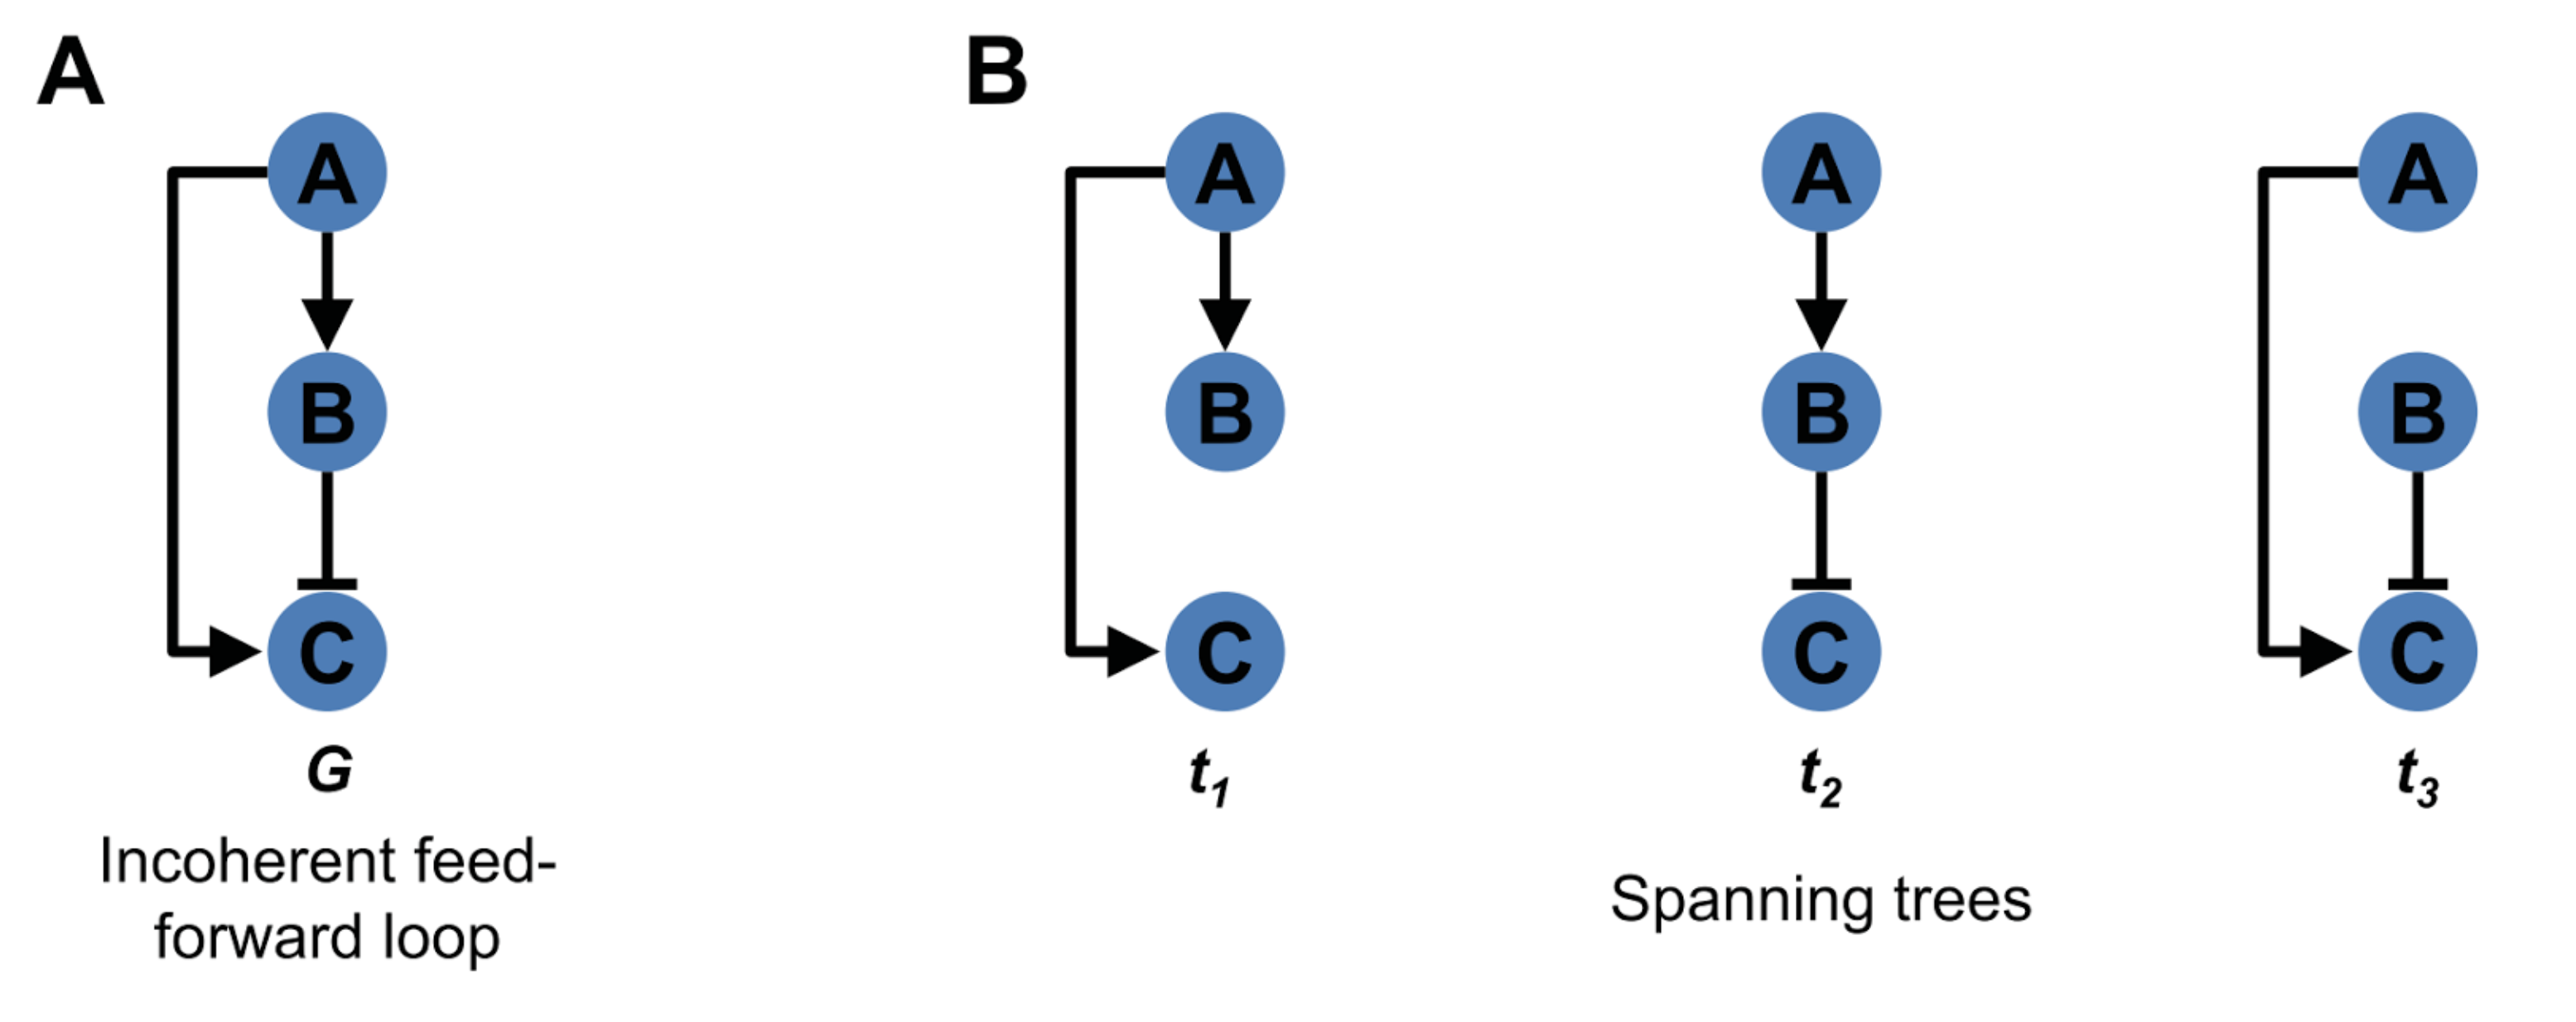
\includegraphics[width=160mm]{figures/sst_example.png}}
\caption[Decomposition of Spanning Trees]{An example decomposition of a small causally inconsistent network A) to its spanning trees B). Figure adapted from~\cite{Vasilyev2014}.}
\label{fig:sst_schematic}
\end{figure}

\subsection{Network Representation Learning}
\label{subsec:nrl}

Representation learning methods have the goal of generating low-dimensional, continuous vector representations for entities in high-dimensional, heterogeneous data sets (e.g., images, text sequences, etc.).
More specifically, network representation learning, also known as \ac{KGE}, learns representations of nodes and edges from \acp{KG} in continuous vector spaces that can be used in downstream machine learning tasks such as edge prediction, entity clustering, and entity disambiguation~\cite{Wang2017}.
Several methods inspired by linear algebra, deep learning, and natural language processing have arisen in previous years as shown in Table~\ref{tab:kgem_examples}.

\begin{table}
    \centering
    \begin{tabular}{ l l l }
        \hline
        Model Type & Name & Reference \\
        \hline
        \multirow{6}{*}{Translational Distance}
        & Structured Embedding & ~\cite{Bordes2011}  \\
        & TransE & ~\cite{Bordes2013} \\
        & Unstructured Model & ~\cite{Bordes2014} \\
        & TransH & ~\cite{Wang2014} \\
        & TransR & ~\cite{Lin2015} \\
        & TransD & ~\cite{Ji2015} \\
        \hline
        \multirow{4}{*}{Semantic Matching}
        & RESCAL & ~\cite{Nickel2011} \\
        & ERMLP & ~\cite{Dong2014} \\
        & DistMult & ~\cite{Yang2014}  \\
        & ConvE & ~\cite{Dettmers2017} \\
        \hline
        \multirow{4}{*}{Random Walk}
        & DeepWalk & ~\cite{Perozzi2014} \\
        & Gat2Vec & ~\cite{Sheikh2018} \\
        & node2vec & ~\cite{Grover2016} \\
        & edge2vec & ~\cite{Gao2018} \\
        & metapath2vec & ~\cite{Dong2017} \\
        & LINE & ~\cite{Tang2015} \\
        \hline
    \end{tabular}
    \caption{Examples of three types of \acp{KGEM}}\label{tab:kgem_examples}
\end{table}

\subsubsection{Translational Distance Models}

Each translational distance model learns entity and relation embeddings in euclidean space by defining two things: 1) an equation relating the corresponding embeddings with the models' hyperparameters and 2) a distance-based measure of the plausibility of a given triple $f_r$~\cite{Wang2017}.

An example of an established translational distance model is TransE~\cite{Bordes2013}.
It models a class of relation \textit{r} as the translation from a head entity $h$ (i.e., the subject of a triple) to a tail entity $t$ (i.e., the object of a triple) in a representative euclidean space as $h + r \approx t$.
It measures the plausibility of a given triple with the following scoring function:

\begin{equation}\label{eq:trans_e_scoring_function}
    f_r(h,t) = - \|h + r - t\|
\end{equation}

The closer the embedding of the tail is to the sum of the head and relation embeddings, the higher is the probability that the triple is correct.
However, because TransE is limited in modeling $1-N$, $N-1$, and to $N-M$ relations, several extensions have been proposed (e.g., TransH, TransR, and TransD).

TransH extends TransE by representing each relation in a relation-specific hyperplane with normal vector $w_r$~\cite{Wang2014}.
Before scoring, the head and tail entities are projected using the following equations before using the same scoring function as in TransE\@.

\begin{equation} \label{eq:trans_h_proj_head}
h_{\perp} = h -w_{r}^\top hw_r
\end{equation}

\begin{equation} \label{eq:trans_h_proj_tail}
t_{\perp} = t -w_{r}^\top tw_r
\end{equation}

Finally, the translation vector $r$ from TransH is constrained to be within the hyperplane defined by $w_r$ before applying the following scoring function.

\begin{equation} \label{eq:trans_h_scoring_function}
    f_r(h,t) = -\|h_{\perp} + r - t_{\perp}\|_{2}^2
\end{equation}

Alternatively, TransR~\cite{Lin2015} and TransD~\cite{Ji2015} use independent projection matricies for the head and tail entities to allow for greater expressibility.
However, these models have more parameters and thus require more data to train well.

\subsubsection{Semantic Matching Models}

Unlike translational distance models, semantic matching models use similarity-based scoring functions that measure the plausibility of a given triple based on the "latent semantics" of the entities and relations~\cite{Wang2017}.
An example of an established semantic matching model is RESCAL~\cite{Nickel2011}.
It represents each entity as a vector and each relation as a matrix, $M_r$, that encodes pairwise interactions between the head and tail entities of a triple, using the following scoring function:

\begin{equation}\label{eq:rescal_scoring_function}
    f_r(h,t) = h^{T} M_{r} t
\end{equation}

The DistMult model simplifies RESCAL by restricting $M_r$ to be a diagonal matrix, denoted as $diag(r)$ in order to reduce the number of model parameters while simultaneously improving the efficiency of computation~\cite{Yang2014}.

\begin{equation} \label{eq:distmult_scoring_function}
    f_r(h,t) = h^{T} diag(r) t
\end{equation}

Both translational distance models and semantic matching models can be trained using the margin ranked loss~\cite{Nickel2016,Dettmers2017} in order to maximize the difference between positive triples (i.e.,~$f_r(h,t)$) and negative ones (i.e.,~$f_r(h^{'},t^{'}$).
This scoring function has the benefits that it can readily integrate a variety of scoring functions $f_r(h, t)$ and it is amenable to the possibility that a negative triple may also be true, but just not included in the knowledge graph.
The margin ranking loss can be optimized with stochastic gradient descent while iterating through batches of positive triples and sampled negative ones~\cite{Bottou2010}.

\begin{equation}\label{eq:margin_ranked_loss}
    L = \sum_{}^{}\max(0, f_r(h^{'},t^{'}) - f_r(h,t) + \lambda)
\end{equation}

\subsubsection{Random Walk Models}

Random walk models generate embeddings for nodes in knowledge graphs by applying the concepts from natural language models (e.g.,~\textit{SkipGram}, \textit{word2Vec}, and \textit{GloVE}) to random walks.

The first, \textit{DeepWalk}~\cite{Perozzi2014}, generates a corpus of random walks from the knowledge graph starting from each node by uniformly randomly choosing an adjacent node at each step in the walk until the target length was achieved or no unvisited neighbors remained.
These walks were used to train the \textit{SkipGram}~\cite{Mikolov2013} model in which the random walks were considered as sentences and nodes were considered as words.
Because \textit{SkipGram} is a language model that maximizes the co-occurrence probability of words in the same window, the node vectors reflect the local structure of the input \ac{KG} (Figure~\ref{fig:deepwalk_embedding}).
It is further rationalized by the observation that the distribution of nodes' appearances in random walks mirrors words in free text~\cite{Perozzi2014}.
Several aspects of knowledge graphs were not addressed by DeepWalk, including the community structure of the second neighbors of each nodes, the types of nodes, the types of edges, and attributes of nodes and edges.

Node2vec~\cite{Grover2016} addresses the community structure of the second neighbors of each node by modifying the random walk process to include second-order random walks, where the probability of walking to each neighbor from a given node is also influenced by its previous steps.
Node2vec has been independently implemented several times, but most suffer from difficulty in implementing second order walking both in terms of algorithmic understandability and from a computational perspective.
Recently, the implementation at \url{https://github.com/VHRanger/graph2vec} has solved many of those issues with both an elegant and efficient implementation.
Edge2vec~\cite{Gao2018} took a similar approach to node2vec by calculating probabilities of traversing each edge type based on the previous steps in a walk.
It was able to better capture the underlying distributions in knowledge graphs with multiple edge types.
Metapath2vec~\cite{Dong2017} created random walks that included the node types and edge types in order to address their absence, and Gat2vec~\cite{Sheikh2018} added attributes as actual nodes to knowledge graphs such that they could be incorporated (and then filtered) from random walks.

Random walk methods are very powerful in that most rely on changing the random walk generation, and the workflow can be maintained.
While it has not yet been done, this leaves significant improvement for abstraction of this methodology and development of powerful and flexible computational frameworks for future research.

\begin{figure}
    \captionsetup{format=plain}
    \makebox[\textwidth]{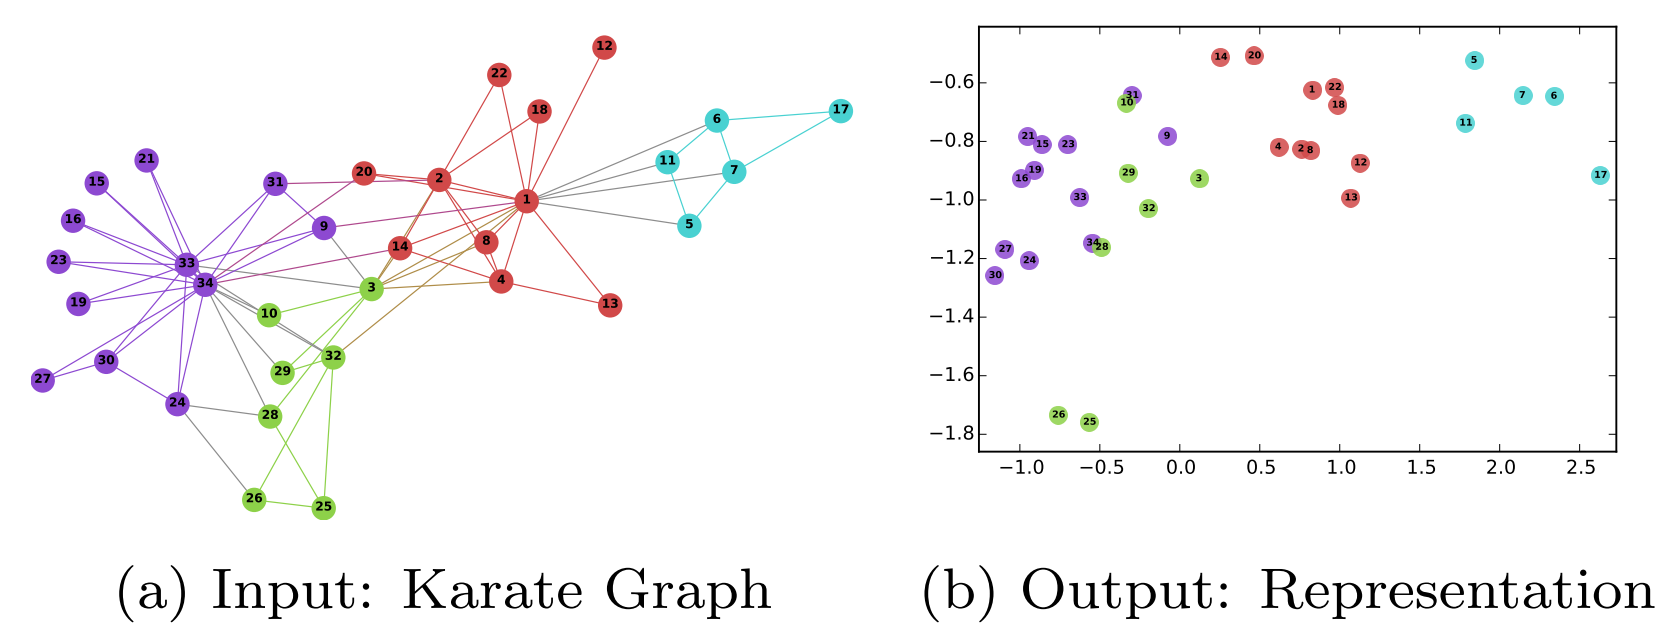
\includegraphics[width=160mm]{figures/deepwalk_embedding.png}}
    \caption[DeepWalk Embeddings Reflect Community Structure]{\textit{DeepWalk} produces embeddings that reflect the community structure of the underlying \ac{KG}. Figure adapted from~\cite{Perozzi2014}}
    \label{fig:deepwalk_embedding}
\end{figure}

\subsubsection{Applicability of Network Representation Learning}

Biological knowledge encoded in many of the previously mentioned formats (e.g., \ac{BioPAX}, \ac{SBML}) can be directly translated into \acp{KG} to which network representation learning can be applied.

Because of the importance of community structure in biological networks~\cite{Girvan2002}, random walk models have the most appropriate formulation for capturing the underlying patterns in biological networks.
A direct comparison for several types of biological networks including protein-protein interaction networks, miRNA-target networks, and other multimodal networks is currently under development following the contribution of related work from this thesis to~\cite{Ali2019}.

The following subsection describes three of such applications in drug discovery.
